%%%%%%%%%%%%%%%%%%%%%%%%%%%%%%%%%%%%%%%%%%%%%%%%%%%%%%%%%%%%%%%%%%%%%%%%%%%%%%%%
%2345678901234567890123456789012345678901234567890123456789012345678901234567890
%        1         2         3         4         5         6         7         8

\documentclass[letterpaper, 11 pt, conference]{ieeeconf}  % Comment this line out
                                                          % if you need a4paper
%\documentclass[a4paper, 10pt, conference]{ieeeconf}      % Use this line for a4
                                                          % paper

\IEEEoverridecommandlockouts                              % This command is only
                                                          % needed if you want to
                                                          % use the \thanks command
\overrideIEEEmargins
% See the \addtolength command later in the file to balance the column lengths
% on the last page of the document



% The following packages can be found on http:\\www.ctan.org
%\usepackage{graphics} % for pdf, bitmapped graphics files
%\usepackage{epsfig} % for postscript graphics files
%\usepackage{mathptmx} % assumes new font selection scheme installed
%\usepackage{times} % assumes new font selection scheme installed
%\usepackage{amsmath} % assumes amsmath package installed
%\usepackage{amssymb}  % assumes amsmath package installed
\usepackage{myPreamble}
\title{\Large \bf Distributed Proportional-Integral Observers for Fault Detection and Isolation
}

%\author{ \parbox{3 in}{\centering Huibert Kwakernaak*
%         \thanks{*Use the $\backslash$thanks command to put information here}\\
%         Faculty of Electrical Engineering, Mathematics and Computer Science\\
%         University of Twente\\
%         7500 AE Enschede, The Netherlands\\
%         {\tt\small h.kwakernaak@autsubmit.com}}
%         \hspace*{ 0.5 in}
%         \parbox{3 in}{ \centering Pradeep Misra**
%         \thanks{**The footnote marks may be inserted manually}\\
%        Department of Electrical Engineering \\
%         Wright State University\\
%         Dayton, OH 45435, USA\\
%         {\tt\small pmisra@cs.wright.edu}}
%}

\author{Sam Nazari$^{1}$ and Bahram Shafai$^{2}$% <-this % stops a space
%\thanks{*This work was not supported by any organization}% <-this % stops a space
\thanks{$^{1}$Sam Nazari is a Ph.D. Candidate at the Department of Electrical and Computer Engineering,
        Northeastern University, Boston MA, USA. 
        {\tt\small nazari@ece.neu.edu}}%.
\thanks{$^{2}$Bahram Shafai is Professor of Electrical and Computer Engineering as well as Biomedical Engineering at Northeastern University, Boston MA, USA.
		{\tt\small shafai@ece.neu.edu}}%
}


\begin{document}



\maketitle
\thispagestyle{empty}
\pagestyle{empty}


%%%%%%%%%%%%%%%%%%%%%%%%%%%%%%%%%%%%%%%%%%%%%%%%%%%%%%%%%%%%%%%%%%%%%%%%%%%%%%%%
\begin{abstract}
This paper considers fault detection and isolation in a distributed setting with agents under consensus dynamics. The distributed fault detection and isolation problem is introduced along with system models to represent nominal and faulty conditions. It is shown that the proportional-integral observer (PIO) effectively estimates the fault signal in an agent and that it can be used for residual generation and fault isolation. The conditions under which fault isolation is achievable are derived as a function of the distributed topology of the agents in the network. An LMI is derived that can be used to conveniently obtain the residual generator gains. The distributed PIO design approach is illustrated with an example. 
\end{abstract}


%%%%%%%%%%%%%%%%%%%%%%%%%%%%%%%%%%%%%%%%%%%%%%%%%%%%%%%%%%%%%%%%%%%%%%%%%%%%%%%%
\section{INTRODUCTION} \label{sec:intro}
Modern society is dependent on interconnected critical infrastructures \cite{teixeira_distributed_2014}. Such large-scale infrastructures comprise of smaller subsystems, referred to as agents, that are interconnected by local information pathways.  Exemplary infrastructures include information networks, financial networks, energy networks, water distribution networks, transportation networks and telecommunication networks. These systems are typically modeled by a collection of agents whose interactions are constrained to involve only a local set of their neighbors, commonly referred to as a distributed system.    

\medskip

Due to recent high profile incidents major emphasis and attention is now being directed at developing rigorous analytic tools to evaluate the vulnerabilities that can lead to unexpected service disruptions in critical infrastructures involving networked control systems (NCS) and Cyber-Physical Systems (CPS) \cite{pasqualetti_control-theoretic_2015,nazari_distributed_2016,teixeira_distributed_2014}. Investigators have turned to systems theory to meet these challenges. In particular, observer theory and its role in fault detection have been fruitful, see \cite{teixeira_distributed_2014} and the references therein. 

\medskip

Since distributed consensus systems lack a centralized monitoring entity, many mission critical applications are prone to disruption from system or component level failures. Faulty agents disrupt the nominal operation of the network, leading to unexpected or erroneous outcomes.  Similarly, component failures in the agents themselves can inject biases into the network leading to undesirable deviations in the network agreement variables. 

\medskip

Traditionally, unknown input observers (UIOs) have been used in fault detection and isolation schemes \cite{chen_robust_1999} and recently, UIOs were considered in distributed fault detection, see \cite{shames_distributed_2011,teixeira_distributed_2014}, for example. In \cite{shames_distributed_2011,teixeira_distributed_2014} the authors address the fault detection and isolation problem by endowing each agent with a UIO to monitor its neighbors for faults. Specifically, they utilize the Generalized Observer Scheme (GOS), where a bank of UIO observers is used to produce a residual signal that can be used to indicate the presence of a faulty agent.  

\medskip

The UIO based GOS is an inherently robust approach but in the distributed case it relies on a bank of observers to produce the signals that make up the generalized residual set. As noted in \cite{shames_distributed_2011}, ``at each node it is required to have one observer corresponding to each of the neighbors. Each of these observers have $2N$ states. So at each node $i$, $2N|N_i|$ states are estimated, which puts a heavy computational burden on each of the nodes as $N$ increases.'' Consequently, in the distributed case, the UIO design demands a heavy computational burden because the system equations must be manipulated so that one column of the fault distribution matrix is expressed as a separate term for uncoupling from the overall system dynamics.   

\medskip

The Proportional-Integral Observer (PIO), on the other hand, directly estimates fault signals along with the system states \cite{oghbaee_complete_2018,shafai_proportional-integral_2015,b._shafai_s._beale_h.h._niemann_and_j._stoustrup_ltr_1996}. This advantageous property leads to a more computationally efficient design in the distributed case since there is no need to uncouple the fault signal from the system states in order to design a residual generator. Furthermore, the PIO structure is directly amenable to residual generation since it estimates the fault signal along with the state vector. Despite its advantages, the PIO has not found widespread use among investigators. During a literature review of distributed PIO, only one reference was found to have considered PIO for use with nonlinear interactions between linear interconnected systems \cite{ghadami_decentralized_2011}. 

\medskip

This paper extends the PIO fault detection theory to to the distributed case. First the fault detection and isolation problem is formulated in terms of distributed agents whose interconnections are constrained by a network topology. It is shown that estimating the state vector of an agents neighbors while performing fault detection and isolation for the same agent is possible using a distributed formulation of the PIO (D-PIO). By using a single D-PIO instead of a bank of observers, it is possible to accommodate simultaneous identification of faults along with reductions in the overall time and space complexity of the distributed fault detection algorithm. 

\medskip

To that end, section \ref{sec:back} provides the mathematical background material.  Section \ref{sec:dpio} states the main detection and identification result. Section \ref{sec:ex} provides an illustrative example and the paper concludes with comments in section \ref{sec:con}.
%%%%%%%%%%%%%%%%%%%%%%%%%%%%%%%%%%%%%%%%%%%%%%%%%%%%%%%%%%%%%%%%%%%%%%%%%%%%%%%%

\section{BACKGROUND} \label{sec:back}
% \subsection{Notation}
% We denote the set of all positive real numbers including zero with the symbol $\Rp = \{x \in \R: x\geq 0\}$. Note that $\Rp$ forms an additive semigroup $(\Rp, +)$ and a multiplicative group $(\Rp, \times)$ with 1 as the natural element. The set $\theta x$ with $\theta \geq 0$ and $x \in \Rp$ forms a cone, denoted by $\mathcal{K}$. A cone $\mathcal{K}$ is a proper cone if it is convex, closed, solid and pointed \cite{boyd_convex_2004}. The nonnegative orthant forms a proper cone which we denote by $\mathcal{K}^n$. For convenience, nonnegative matrices are denoted by $M \geq 0$. We use similar notation for vectors and scalars. Relatedly, we use the notation $M > 0$ to mean the matrix $M$ with entries that are strictly positive. We reserve the symbol $\succeq$ refer to positive semi-definite matrices, \eg $P \succeq 0$. 
\subsection{Graph Theory}
Graph theory has been used to model the interconnected nature of many networked control systems, multi-agent systems and cyber-physical systems. In this section, the rudiments of graph theory are reviewed. The interested reader is referred to \cite{godsil_algebraic_2013} for an elaborate treatment.

\medskip

A graph shall be denoted by $\cG = (\mathcal{V},\mathcal{X})$, where $\mathcal{V} = \{1,\ldots, n\} \in \mathbb{N}$ is the \textit{vertex set} and $\mathcal{X} \subseteq \mathcal{V} \times \mathcal{V}$ is the \textit{edge set}. It is assumed all graphs are finite, simple and connected.  Denote by $xy \in \mathcal{X}$ the edge $xy$ that is in the edge set of the graph $\cG$. In this case, $x$ and $y$ are considered to be \textit{adjacent or neighboring} vertices.  If all the vertices of $\cG$ are pairwise adjacent, then $\cG$ is complete.  A complete graph on $n$ vertices is denoted by $K_n$.  If $\cG$ is an undirected graph and a subset of the vertices, $S \subset \cV$, forms a complete graph, then the subgraph induced by $S$ is known as a \textit{clique}. The number of vertices in a graph known as the graph \textit{order}, usually denoted by $|\cG|=n$. The vertex, $a \in \cV$, is \textit{incident} with the edge, $e=(c,a)$, if $a \in \cV$ participates in $e$.  Then it is said that $e$ \textit{joins} $c \in \cV$ and $a \in \cV$, the \textit{endvertices}.

\medskip

The set of \textit{neighbors} of the vertex $a \in \cV$ is denoted by $\mathcal{N}_a$. The notation $|\mathcal{N}_a|=m$ denotes the cardinality of the set of neighbors of $a \in \cV$, in this case $m$. The \textit{degree} of a vertex $a \in \cV$ is the number of edges that the vertex $a \in \cV$ participates in $d_a := |\{b: (ab) \in \mathcal{X}\}|$. If every vertex has the same degree, $d$, then we say $\cG$ is a $d$-\textit{regular} graph and denote this by $\cG_d$. 

\medskip 

Consider $\cG = (\mathcal{V},\mathcal{X})$. Define a map from the vertex space of $\cG$ to the reals, $x: \mathcal{V} \rightarrow \mathbb{R}$. Similarly, define a map from the edge space of $\cG$ to the reals, $y: \mathcal{X} \rightarrow \mathbb{R}$. The mappings $x$ and $y$, associate with each vertex (or edge) a scalar numeric value from the reals. Fix $|\cV|=n$ and consider the linear operator $\cA:\mathbb{R}^n \rightarrow \mathbb{R}^n$. When $\cA$ is applied to $x$, the resulting value at a vertex $a \in \cV$ is the sum of the values of the function $x$ over all the neighbors, $b \in \mathcal{N}_a$, of $a \in \cV$.  Hence the action of the operator $\cA$ on $x$ at $a \in \cV$ can be captured as $(\cA x)(a) = \sum_{b:(ab) \in \mathcal{X}} x(b)$. $\cA$ will be referred to as the \textit{adjacency matrix} of $\cG$, usually defined by
\begin{align*}
 \cA_{ij}= 
\begin{cases}
    1,              & \text{if } ij\in \mathcal{X}\\
    0,              & \text{otherwise}
\end{cases}
\end{align*}
Relatedly, define the Laplacian matrix $\cL$ of a graph as the quantity that measures the smoothness of $x$ over the edges of $\cG$ \cite{spielman_spectral_2011}. This notion is most easily seen from inspection of the quadratic form that $\cL$ induces
\begin{align*}
x^T \cL x = \sum_{ab \in \cE} \left( x(b) - x(a) \right )^2.
\end{align*}
By inspection it can be seen that the Laplacian quadratic form provides a sense of the relative smoothness of the function $x$ over the graph $\cG$. The Laplacian matrix of $\cG$ is commonly defined as
\begin{align*}
\cL = \cD - \cA = 
\begin{cases}
d_i, & \text{if } i = j \\
-1,  & \text{if } ij \in \cE \\
0,   & \text{otherwise.}
\end{cases}
\end{align*}
where $\cD$ is a diagonal matrix with entries corresponding to the row sums of the graph adjacency matrix. The Laplacian matrix of $\cG$ has many notable properties.  Here, it is only noted that $\cL$ is a symmetric, positive semidefinite, diagonally dominant, M-matrix. 

% \medskip

% To simplify some of the analysis, this paper considers only $d$-regular graphs $\cG_d$. In $d$-regular graphs, it is slightly more convenient to work with its normalized adjacency matrix
% \begin{align*}
% \cM = \frac{1}{d}\cA
% \end{align*}
% for which we have the following relation
% \begin{lemma} \label{lem:eigA}
% Let $\cG_d$ be a finite, simple, $d$-regular graph and let $\cM \in \R^{n \times n}$ be its normalized adjacency matrix. Let 
% \begin{align*}
% \mu_1 \geq \mu_2 \geq \ldots \geq \mu_n
% \end{align*}
% be the real eigenvalues of $\cM \in \R^{n \times n}$ with multiplicities. Then, 
% \begin{enumerate}
% \item $\mu_1 = 1$ and $\mu_n \geq -1$.
% \item $\mu_2 = 1$ if and only if $\cG_d$ is disconnected.
% \item $\mu_n = -1$ if and only if at least one of the connected components of $\cG_d$ is bipartite.
% \end{enumerate}
% \end{lemma}
% \begin{proof}
% The reader is referred to \cite{godsil_algebraic_2013} for the proof.
% \end{proof}
% Similarly, in the setting of a $d$-regular graph, it is slightly more convenient to work with the normalized Laplacian matrix
% \begin{align*} 
% \cQ = I-\cM
% \end{align*}
% for which we have the following relation
% \begin{lemma} \label{lem:eigL}
% Let $\cG_d$ be a finite, simple, $d$-regular graph and let $\cQ \in \R^{n \times n}$ be its normalized Laplacian matrix. Let 
% \begin{align*}
% \lambda_1 \leq \lambda_2 \leq \ldots \leq \lambda_n
% \end{align*}
% be the real eigenvalues of $\cQ \in \R^{n \times n}$ with multiplicities. Then, 
% \begin{enumerate}
% \item $\lambda_1 = 0$ and $\lambda_n \leq 2$.
% \item $\lambda_k = 0$ if and only if $\cG_d$ has $k$ connected components.
% \item $\lambda_n = 2$ if and only if at least one of the connected components of $\cG_d$ is bipartite.
% \end{enumerate}
% \end{lemma}
% \begin{proof}
% The reader is referred to \cite{godsil_algebraic_2013} for the proof.
% \end{proof}
\subsection{Proportional-Integral Observer for Fault Detection} 
The problem of designing observers for a linear systems has been studied since Luenberger introduced the Luenberger observer in the 1960's. There are many observer structures, the reader is referred to \cite{oreilly_observers_1983} and the references therein for more information. This paper considers systems that can be modeled by equations of the following form: 
\begin{gather}
\begin{aligned} \label{eq:eq1}
\dot{x}(t) &= Ax(t) + Bu(t) + E f (t) \\
y(t) &= Cx(t) + Du(t)
\end{aligned}
\end{gather}
where $x(t) \in \R^n$ is the system state vector, $u(t) \in \R^m$ is the system input, $y(t) \in \R^p$ is the system output, $f(t) \in \R^{q}$ is a constant (\ie $\dot{f}(t)=0$) actuator fault vector and $A \in \R^{n \times n}$, $B \in \R^{n \times m}$, $C \in \R^{p \times n}$, $E \in \R^{n \times q}$ with $D=0$ for the remainder of the paper without loss of generality. The following conditions for the system in (\ref{eq:eq1}) are assumed throughout the rest of the paper:
\begin{ass} \label{ass:minRep}
The system (\ref{eq:eq1}) is controllable and observable, \ie that (\ref{eq:eq1}) is a minimal realization of the actual system being modeled.
\end{ass}
\begin{ass} \label{ass:ass1}
$\rho(C) = p$ (\ie $C$ is full row rank) and $\rho(E) = q$ (\ie $E$ is full column rank) and furthermore that $\rho(CE) = \rho(E)$.
\end{ass}
\begin{ass} \label{ass:ass2}
For every $\lambda$ with non-negative real part 
\begin{align*}
\rho \left ( \left [ \begin{array}{cc} A-\lambda I&E \\ C&0 \end{array}\right ] \right )= n + q.
\end{align*}
\end{ass}
Under assumptions \ref{ass:minRep}-\ref{ass:ass2}, a PIO for the system in (\ref{eq:eq1}) is defined by 
\begin{gather}\label{eq:eq2}
\begin{aligned} 
\dot{\hat{x}}(t) &= (A-L_P C)\hat{x}(t) + Bu(t) + L_P y(t) + E \hat{f}(t) \\
\dot{\hat{f}}(t) &= L_I (y(t) - C\hat{x}(t)),
\end{aligned}
\end{gather}
where $\hat{x}(t) \in \R^n$ is the state estimate, $\hat{f}(t) \in \R^q$ is the estimated fault signal, $L_P \in \R^{n \times p}$ is the proportional gain and $L_I \in \R^{q \times p}$ is the integral gain. The structure of the PIO is shown in Figure \ref{fig:PIO} below.
\begin{figure}[H]
    \centering
    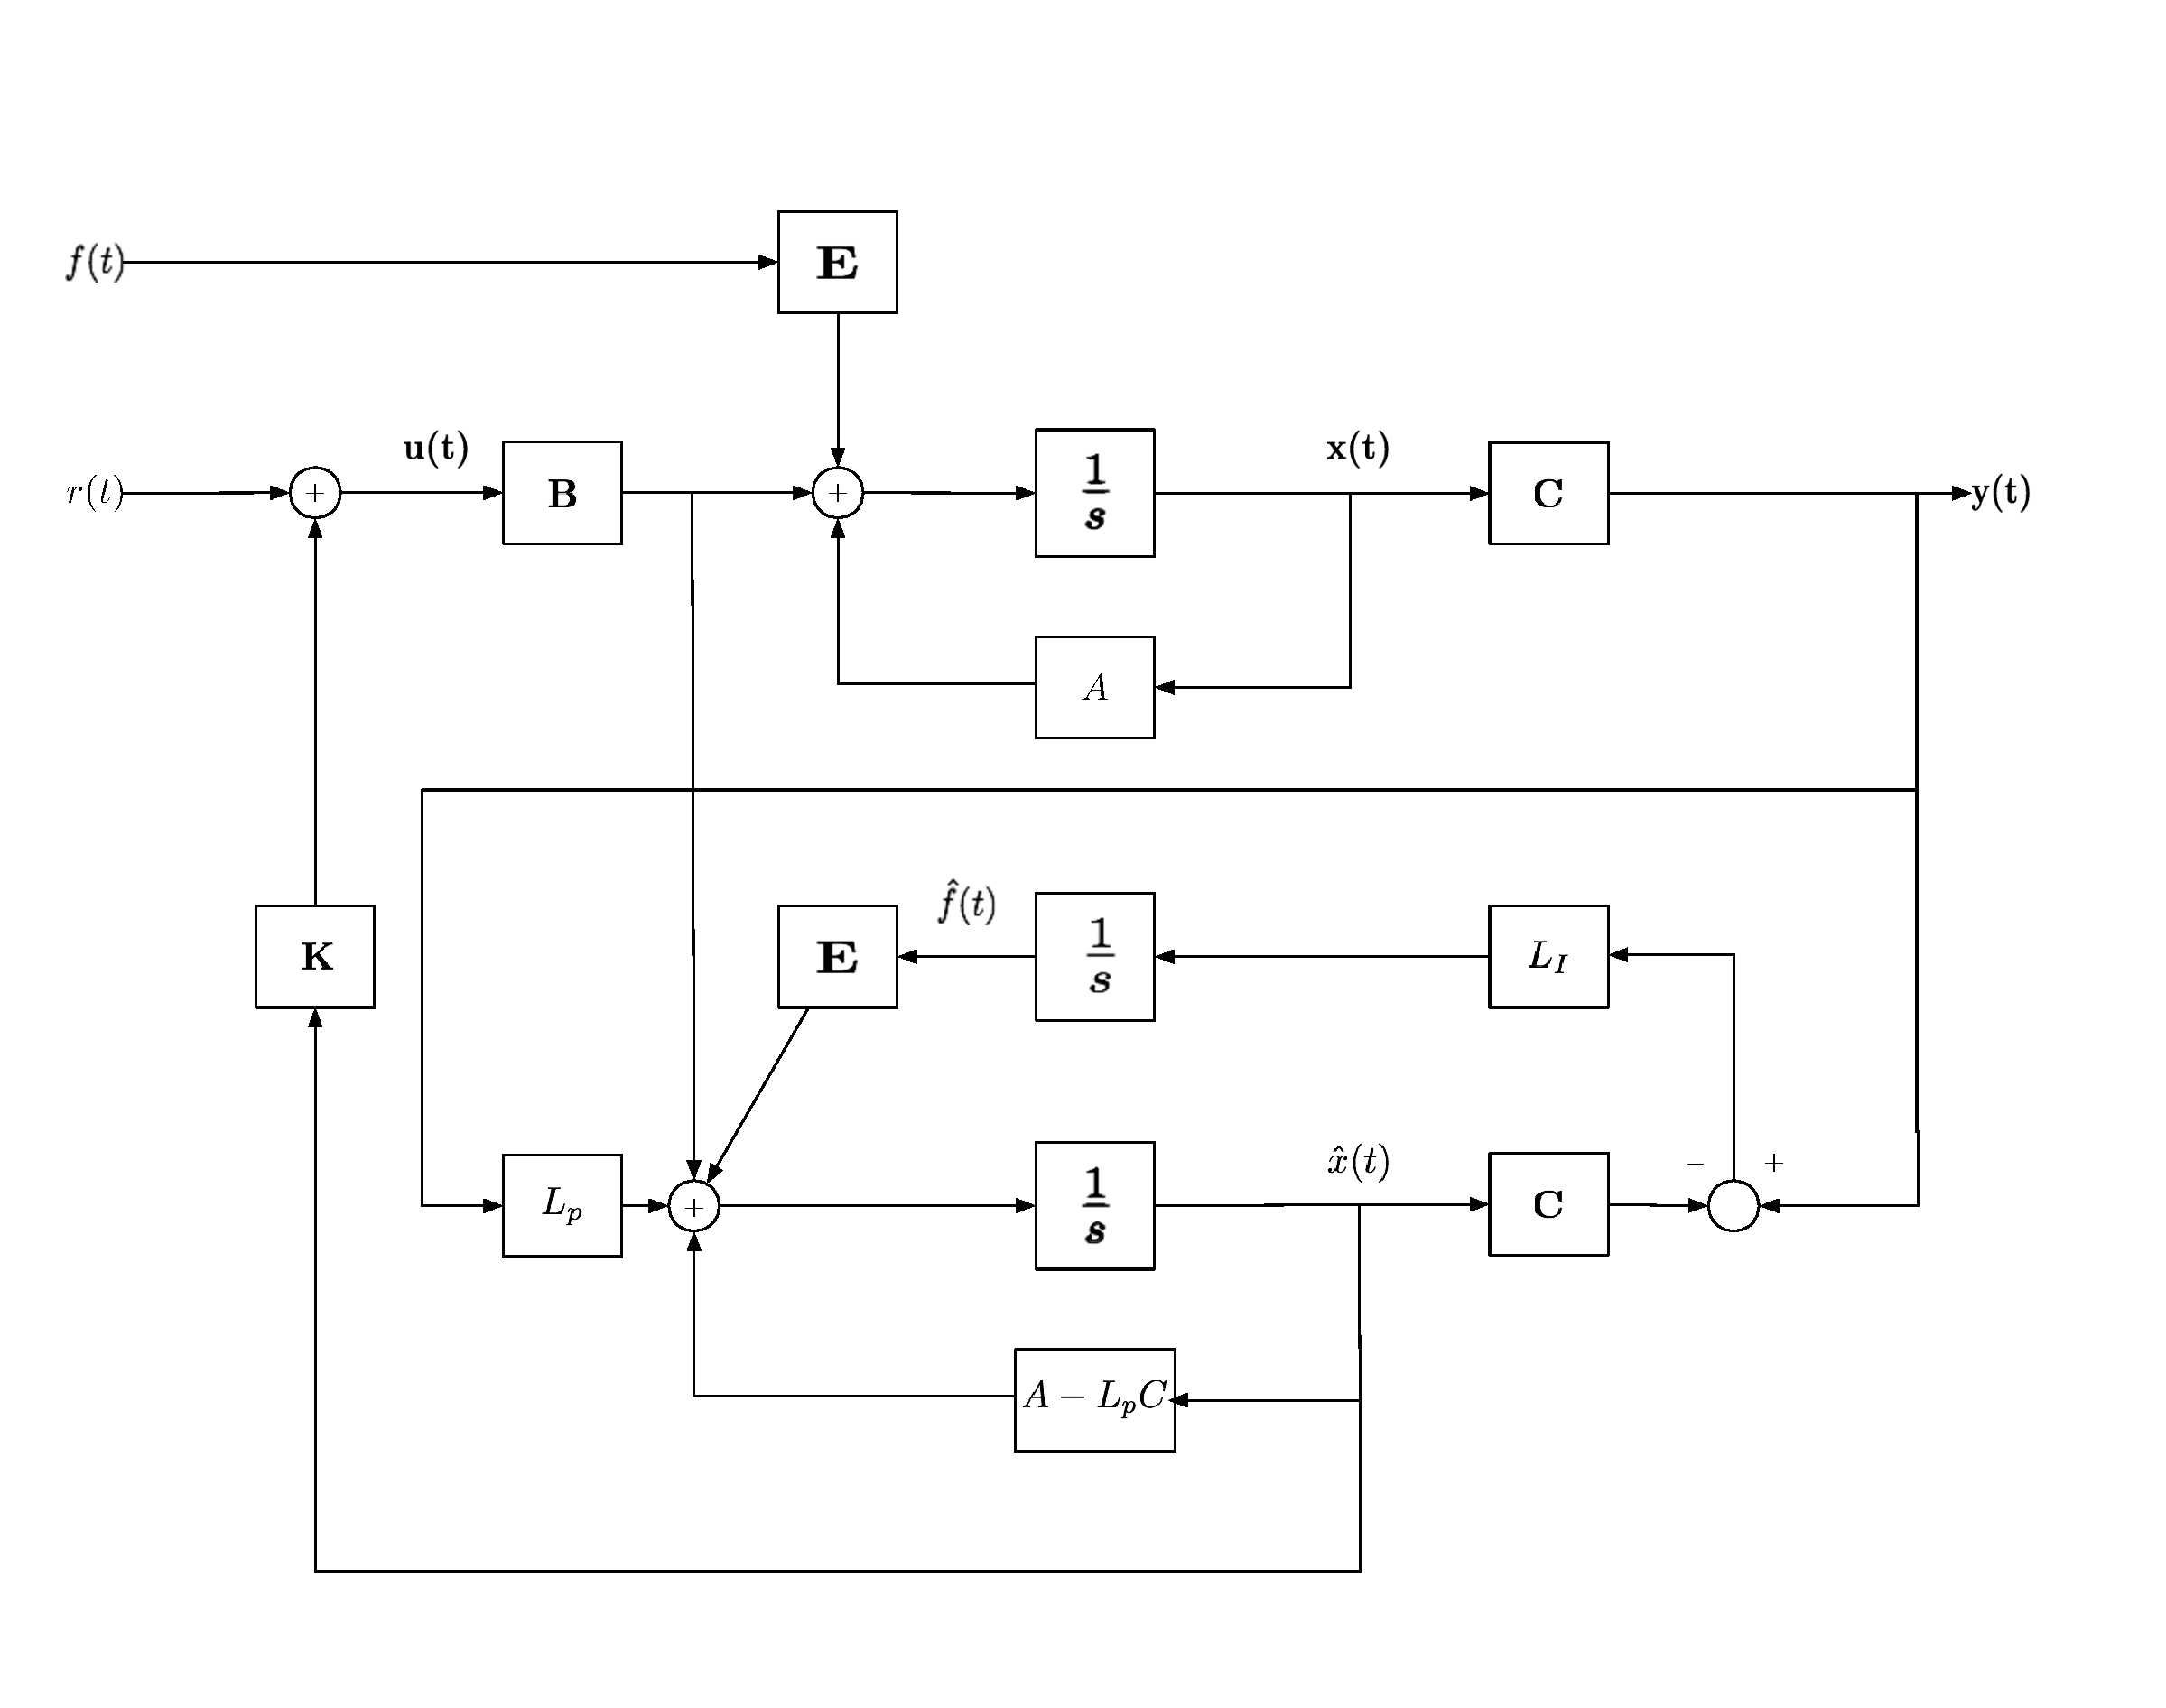
\includegraphics[scale=0.22]{images/PIO_FDIR.pdf}
    \caption{The PIO structure for simultaneous state and fault estimation.}
    \label{fig:PIO}
\end{figure}
\begin{theorem} \label{thrm:thrm1}
Under assumptions (\ref{ass:minRep}-\ref{ass:ass2}), the PIO (\ref{eq:eq2}) is an asymptotic state estimator for the system given in (\ref{eq:eq1}) with estimator gains given by eigenvalue assignment of $A_x - L_x C_x$, where 
\begin{align*}
A_x = \left [ \begin{array}{cc} A & E \\ 0 & 0 \end{array} \right ], 
L_x = \left [ \begin{array}{c} L_p \\ L_I \end{array} \right], 
C_x = \left [\begin{array}{cc} C & 0 \end{array} \right ] 
\end{align*}
or equivalently through the feasible solution of the following LMI:
\begin{align} \label{eq:eq3}
A_x^{\tT} P_x - C_x^{\tT}G_x^{\tT}+P_x A_x - G_x C_x  < 0 
\end{align}
where $G_x = P_x L_x$. 
\end{theorem}
\begin{proof}
To begin, note that by assumption \ref{ass:ass1} the pair $\{A,C\}$ is observable which leads to the fact that for any suitable matrix gain $L$ the eigenvalues of the stable matrix $A-LC$ can be shifted as desired. Consequently, to prove this result define $\tilde{x}(t) = x(t) - \hat{x}(t)$ and $\tilde{f}(t) = f(t) - \hat{f}(t)$ and let the new state vector be $\phi(t) = [ \tilde{x}(t)^{\tT} \tilde{f}(t)^{\tT} ]^{\tT}$. A Lyapunov equation for this system can be fashioned by
\begin{align} \label{eq:lyapunov}
V = \phi^{\tT} P_x \phi.
\end{align}
where we have dropped the time dependence for notational expediency. Taking the time derivative of (\ref{eq:lyapunov}), we seek $\dot{V} < 0$
\begin{align*}
\dot{V} &= \dot{\phi}^{\tT} P_x \phi + \phi^{\tT} P_x \dot{\phi} \\
        &= (A_x - L_x C_x)^{\tT}P_x + P_x (A_x - L_x C_x) < 0
\end{align*}
which reduces to (\ref{eq:eq3}) with the substitution $G_x = P_x L_x$. 
\end{proof}
%%%%%%%%%%%%%%%%%%%%%%%%%%%%%%%%%%%%%%%%%%%%%%%%%%%%%%%%%%%%%%%%%%%%%%%%%%%%%%%%

\section{Distributed Fault Detection and Isolation} \label{sec:dpio}
\subsection{Distributed System Models}
% \textcolor{red}{Note that: $L \in \mathbb{R}^{n \times n}$, $x \in \mathbb{R}^n$, $y \in \mathbb{R}^m$, $C_i \in \mathbb{R}^{m\times n}$, $b_j \in \mathbb{R}^n$, $D_i \in \mathbb{R}^{n \times m}$ and that $|\mathcal{N}_i| = k$.}
\subsubsection{Nominal Dynamics} Consider a group of $n$ agents with state $\psi_i(t)$ having single integrator dynamics 
\begin{gather} 
\begin{aligned}
\dot{\psi}_i(t) &= u_i(t) + v_i(t), \quad \psi_i (0) = \psi_{i0} \in \R \nonumber \\
y_i(t) &= \psi_i (t) \nonumber
\end{aligned}
\end{gather}
where $v_i(t)$ is a known scalar input. The underlying interactions of such a interconnected system can be modeled by an undirected graph, $\cG = (\mathcal{V},\mathcal{X})$ \cite{olfati-saber_consensus_2007}. Let the first-order consensus law 
\begin{align}
u_i(t) = \sum_{j \in \mathcal{N}_i} (\psi_j(t) - \psi_i(t)) \nonumber
\end{align}
be assumed; where $u_i(t)$ is the control input to agent $i \in \mathcal{V}$, $\psi_i(t) \in \mathbb{R}$ is the state of agent $i$ and $\psi_j(t) \in \mathbb{R}$ is the state of agent $i$'s neighbor. In the case where there are no faults or disturbances, the model 
\begin{gather} 
\begin{aligned} \label{eq:agentCons}
\dot{\psi}_i(t) &= \sum_{j \in \mathcal{N}_i} (\psi_j(t) - \psi_i(t)) +v_i (t) \\
y_i(t) &= \psi_i(t) \nonumber
\end{aligned}
\end{gather}
is valid for each agent $i \in \mathcal{V}$. Under these assumptions, the collective dynamics of the entire network are given by \cite{olfati-saber_consensus_2007}:
\begin{align} \label{eq:eq4}
\dot{\mathbf{x}}(t) =-\cL\mathbf{x}(t) + \cB \mathbf{v} (t)
\end{align}
where $\cL \in \mathbb{R}^{n \times n}$ is the graph Laplacian of $\cG$ and $\mathbf{x}(t) \in \mathbb{R}^n$ is the (collective) state vector, $\cB \in \R^{n \times n}$ is a diagonal matrix that is taken to be the $n \times n$ identity matrix in this paper and $\mathbf{v}(t) \in \R^n$ is a vector with known elements. In a distributed system, each agent $i \in \mathcal{V}$ only has access to the states of the $|\cN_i|$ agents in its local neighborhood. Let the set of states available to agent $i \in \mathcal{V}$ be defined by:
\begin{align} \label{eq:eq5}
w_i(t) = \left [ \begin{array}{ccc} \psi(t)_{i_1},&\ldots,&\psi(t)_{i_{|\mathcal{N}_i}|} \end{array}\right ]^{\tT} = \cC_i \mathbf{x}(t) 
\end{align}
where $\cC_i \in \mathbb{R}^{p \times n}$ encodes the interconnection topology of agent $i \in \mathcal{V}$. 
\subsubsection{Faulty Dynamics} In the presence of faults, the system model for the agent that is subject to the fault must be modified since it no longer updates its state according to the consensus protocol. Instead, if agent $j \in \mathcal{N}_i$ experiences an fault, then it may update its state according to:
\begin{gather} 
\begin{aligned} %\label{eq:agentConsFaultAct}
\dot{\psi}_j(t) &= \sum_{i \in \mathcal{N}_j} (\psi_i(t) - \psi_j(t))+v_j (t) + f_j(t) \nonumber \\
y_j(t) &= \psi_j(t)
\end{aligned}
\end{gather}
where $f_j(t)$ is a function of time that is due to the fault signal. 
\begin{definition}
(Faulty Agent): Agent $j \in \mathcal{N}_i$ is said to be a \textit{faulty} agent if $f_j(t) \neq 0$ in (\ref{eq:eq5}) for all time. 
\end{definition}
The network dynamics now become \cite{teixeira_toward_2014}:
\begin{gather} \label{eq:eq6}
\begin{aligned} 
\dot{\mathbf{x}}(t) &= -\cL\mathbf{x}(t)+\cB \mathbf{v}(t) + \cE \mathbf{f}(t) \\
\mathbf{y}(t) &= \mathbf{x}(t)
\end{aligned}
\end{gather}
 where $\cE \in \mathbb{R}^{n \times q}$ is the fault distribution matrix that is a function of the graph topology and $\mathbf{f}(t) \in \R^q$ is a vector of faults that occur at $t$. %If, instead, agent $j$ is 
\subsection{Residual Generator and Fault Isolation with PIOs}
In order to perform fault isolation it is necessary to distinguish various classes of faults from one another. The traditional method is to utilize the structured residual set \cite{chen_robust_1999}. In this approach, fault isolation is achieved using a set of structured residuals.  Every residual in the set is designed to be sensitive to a subset of the faults and insensitive to everything else. 

\medskip

In a distributed system, fault isolation amounts to identifying the set of neighboring nodes that have experienced a fault based on a threshold that is exceeded by a residual signal. In this setting, each neighboring agent represents a fault class. The residual generator is embedded in the monitoring agent, which is selected by the designer. The residual signal is traditionally a function of the state estimate. In a PIO based design, the residual signal is immediately available through the observer estimate. This is because the fault signal $\hat{f}_i (t)$ is also estimated along with the state vector. Therefore, no additional step is required to form a residual generator. The main result of the paper is now stated followed by some remarks. 
\begin{figure}
    \centering
    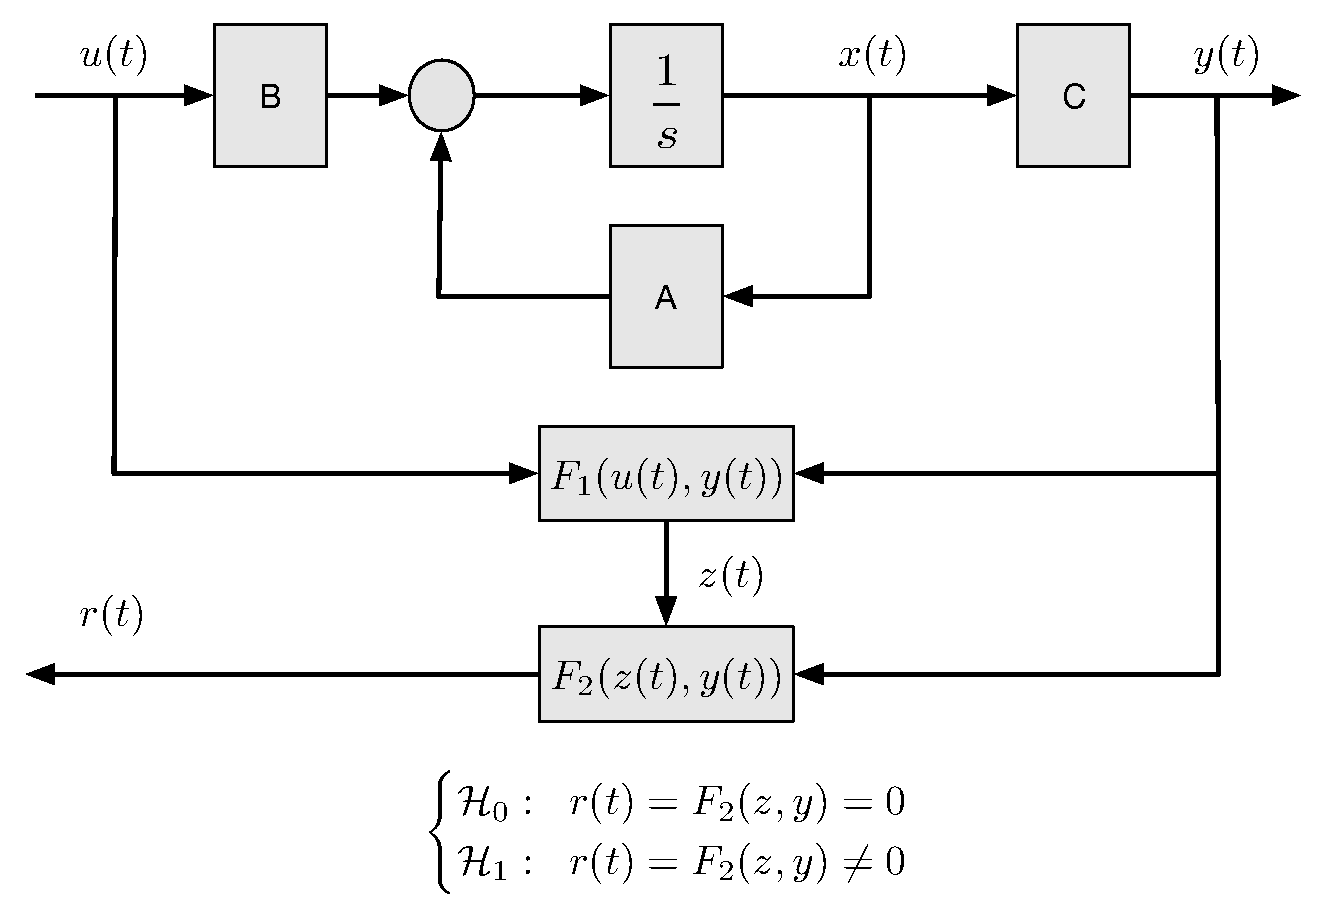
\includegraphics[scale=0.4]{images/FDIframework.pdf}
    \caption{A general residual generator for a linear system. The residual signal, $r(t)$ is shown as $F_2(z(t),y(t))$. Though not shown here, the residual generator may also be a function of the system input $u(t)$.}
    \label{fig:GenericFDIFramework}
\end{figure}
\begin{theorem}
For a distributed system with nominal consensus dynamics given by (\ref{eq:eq5}) 
% \begin{align*} 
% \dot{\mathbf{x}}(t) &=-\cL \mathbf{x}(t) + \cB \mathbf{v}(t)
% \end{align*}
and faulty dynamics of agent $i \in \cV$ given by (\ref{eq:eq7}),
% \begin{align} \label{eq:agentFaults}
% \dot{\mathbf{x}}(t) &= -\cL \mathbf{x}(t)+\cB \mathbf{v}(t) + \cE \mathbf{f}(t)
% \end{align}
a D-PIO of the form
\begin{gather} \label{eq:eq7}
\begin{aligned}
\dot{\hat{\mathbf{x}}}(t) &= \left ( -\cL - L_{P} \cC_i \right ) \hat{\mathbf{x}}(t) + L_{P} w_i(t) + \cB \mathbf{v}(t) + \cE\hat{\mathbf{f}} (t) \\
\dot{\hat{\mathbf{f}}} (t) &= L_{I_i} (w_i (t) - \cC_i\hat{\mathbf{x}} (t))
\end{aligned}
\end{gather}
exists if and only if
\begin{enumerate}
\item the pair $\{ -\cL, \cC_i \}$ is observable, 
\item the rank conditions $\rho(\cC_i) = \rho (\cE) = |\cN_i|$ and $\rho(\cE) = \rho(\cC_i \cE)$ are satisfied, and 
\item for every $Re (\lambda) > 0$ 
\begin{align*}
\rho \left ( \left [ \begin{array}{cc} -\cL - \lambda I & \cE \\ \cC_i & 0 \end{array} \right ] \right ) = n+q. 
\end{align*}
\end{enumerate}
Furthermore, if the conditions (1-3) above are met then a residual generator for agent $i$ can be constructed based on (\ref{eq:eq7}) with gains that are obtained by the feasible solution to the following LMI
\begin{align} \label{eq:eq8}
\cA_x^{\tT} \cP_x -\cC_x^{\tT}\cK_x^{\tT} + \cP_x \cA_x - \cK_x \cC_x < 0  
\end{align}
where $\cK_x = \cP_x L_x$ and 
\begin{align*}
\cA_x = \left [ \begin{array}{cc} -\cL & \cE \\ 0 & 0 \end{array} \right ], 
L_x = \left [ \begin{array}{c} L_{P} \\ L_{I} \end{array} \right], 
\cC_x = \left [\begin{array}{cc} \cC_i & 0 \end{array} \right ].
\end{align*}
\end{theorem}
\smallskip
\begin{proof}
The line of this proof follows the same as the proof from theorem \ref{thrm:thrm1}. 
% Let 
% \begin{align*}
% \cA_x = \left [ \begin{array}{cc} -\cL & \cE \\ 0 & 0 \end{array} \right ], 
% \cB_x = \left [ \begin{array}{c} B \\ 0 \end{array} \right ],
% \cC_x = \left [\begin{array}{cc} \cC_i & 0 \end{array} \right ]
% L_x = \left [ \begin{array}{c} L_{P_i} \\ L_{I_i} \end{array} \right], 
% \end{align*}
\end{proof}
\begin{remark}
Condition 1 in theorem \ref{thrm:thrm1} is needed in order to obtain a valid observer gain and condition 2 establishes the observability of a fault in a local neighborhood of the monitoring agent. Finally, condition 3 relates the graph topology and the fault observability. 
\end{remark}
\begin{remark}
If necessary it is possible to avoid the application of (\ref{eq:eq8}) since eigenvalue assignment on $\cA_x-L_x \cC_x$ will result in a valid residual signal also.
\end{remark}
%%%%%%%%%%%%%%%%%%%%%%%%%%%%%%%%%%%%%%%%%%%%%%%%%%%%%%%%%%%%%%%%%%%%%%%%%%%%%%%%

\section{EXAMPLE} \label{sec:ex}
This example illustrates the residual generator design for agent 1 shown in Figure \ref{fig:graph}. Agent 1 has a neighborhood composed of agents $\{2,3,4\}$. Therefore, the residual generator will generate three residual signals to be monitored. Each signal represents a fault in the associated neighboring node. Based on the interconnection topology of the graph in Figure \ref{fig:graph}, the Laplacian of the graph is found to be
\begin{align*}
\cL = \left [\begin{array}{ccccccc} 
	3&-1&-1&-1&0&0&0\\
    -1&4&-1&-1&-1&0&0\\
    -1&-1&3&0&0&-1&0\\
    -1&-1&0&3&0&0&-1\\
     0&-1&0&0&2&0&-1\\
     0&0&-1&0&0&2&-1\\
     0&0&0&-1&-1&-1&3 \end{array} \right ]
\end{align*}
The local interconnection neighborhood of agent 1 is obtained to be
\begin{align*}
C_1 = \left [ \begin{array}{ccccccc} 
     0&1&0&0&0&0&0\\
     0&0&1&0&0&0&0\\
     0&0&0&1&0&0&0 \end{array} \right ].
\end{align*}
Note that $\rho(C_1) = 3$, $\rho(\cE) = 1$ and $\rho(C_1\cE) = 1$. Hence, we obtain $L_P$ and $L_I$ as

\begin{align*}
L_{P_1} = \left [ \begin{array}{ccc} 
    1.4258&    1.3753&    0.5887\\
    2.6642&    1.5090&    0.1192\\
    1.5106&    3.2990&   -0.2920\\
    0.3865&    0.0854&    2.0368\\
    1.2235&    0.1129&   -0.1426\\
    0.1022&    1.0379&    0.0234\\
    -0.1241&    0.0334&    0.8533 \end{array} \right ], L_I = 10.
\end{align*}
With the gains in hand, we proceed to design the D-PIO, which is able to simultaneously estimate the state and the fault signal. For this numerical example, we chose to inject a step function as the actuator fault at $t = 2$ seconds. As shown in the first plot of figure \ref{fig:D_PIO_1}, the state estimation error shows a quick transient at $t = 2$ seconds which quickly decays back down to zero. The disturbance estimate is shown in figure \ref{fig:D_PIO_2} and it can be seen that the disturbance estimate corresponding to agent 2 quickly changes its mean value for $t>2$ seconds. A suitable detection threshold can be found so that the fault estimate can be used as a residual generator with isolation capabilities as can be seen in figure \ref{fig:D_PIO_2}. Finally, note that although the distributed system in this example is of order 7, the monitoring agent 1 only has access to observations from its local neighborhood, which consists of three agents. Therefore $|\cN_i| = 3$ and the residual generator is able to isolate the source agent with the fault. 
\begin{figure}
    \centering
    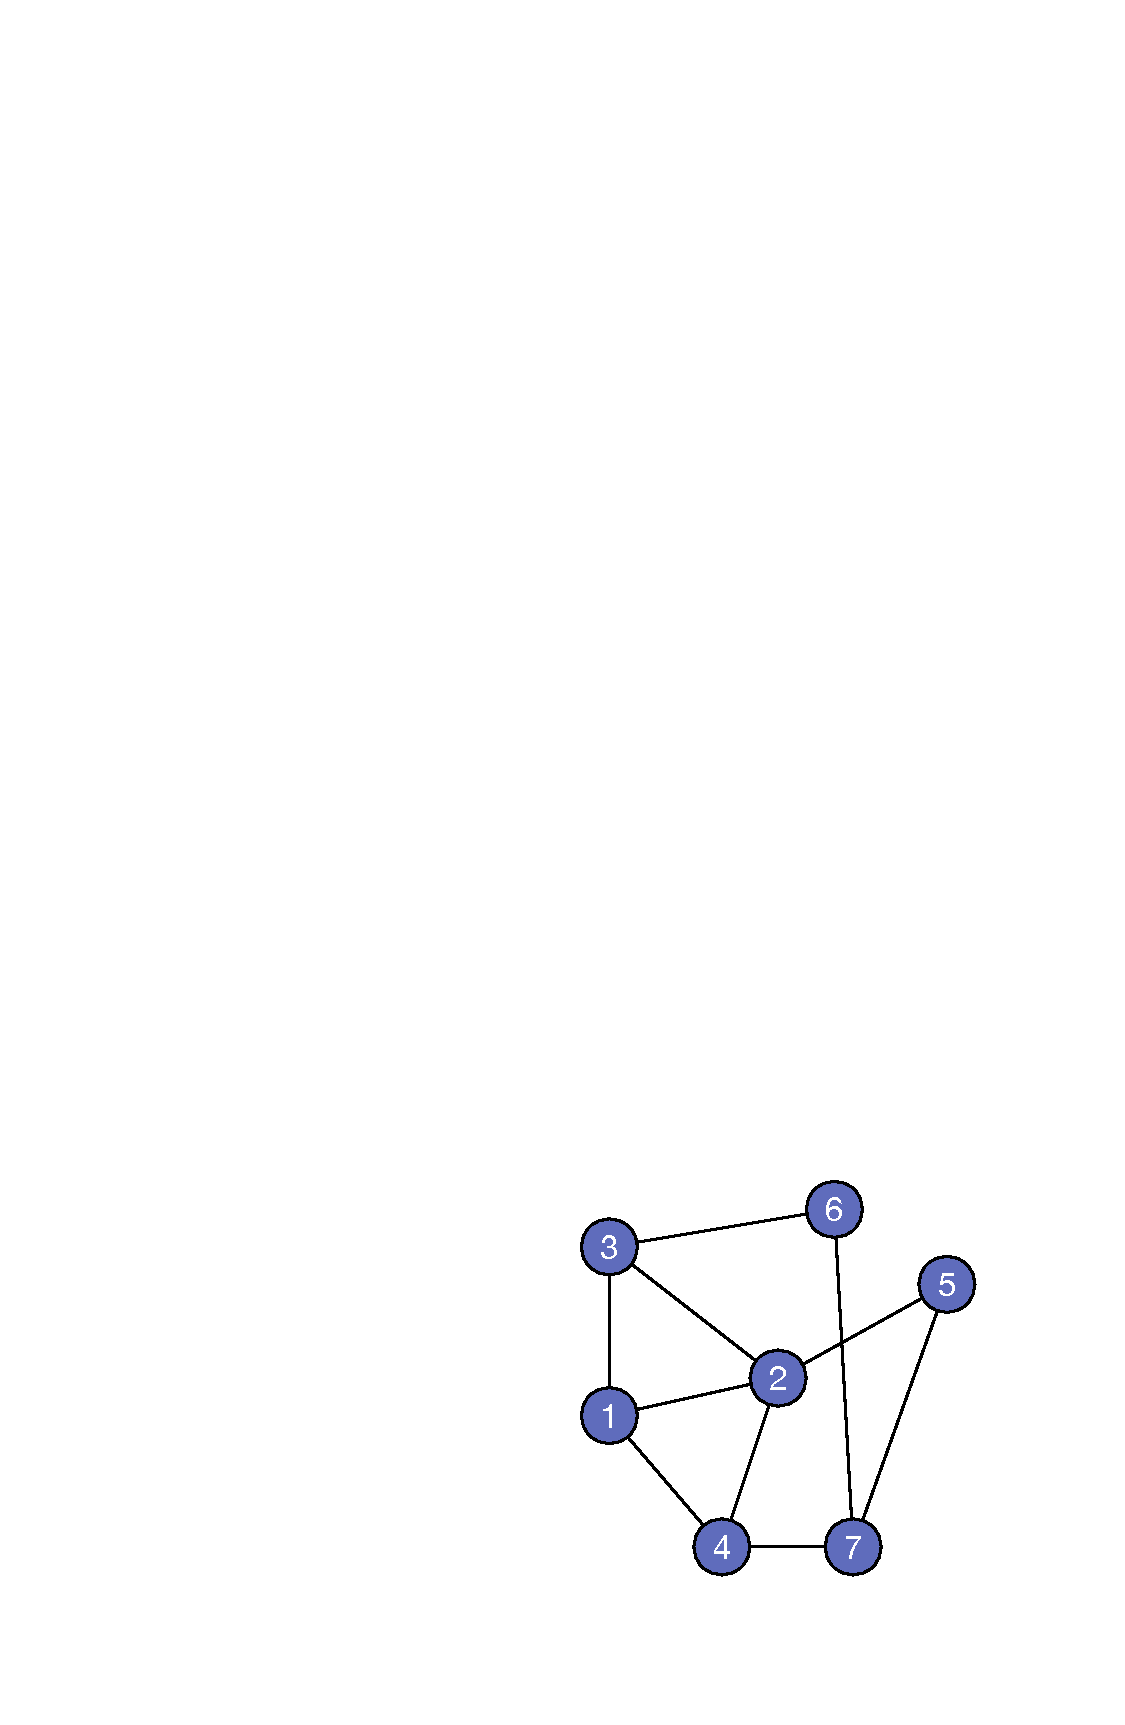
\includegraphics[scale=0.5]{images/CCTA.pdf}
    \caption{Graph representing the underlying interconnections between agents under consideration in example 1. Agent 1 is endowed with a PIO based residual generator which monitors agents 2,3 and 4 for faults.}
    \label{fig:graph}
\end{figure}
\begin{figure}
    \centering
    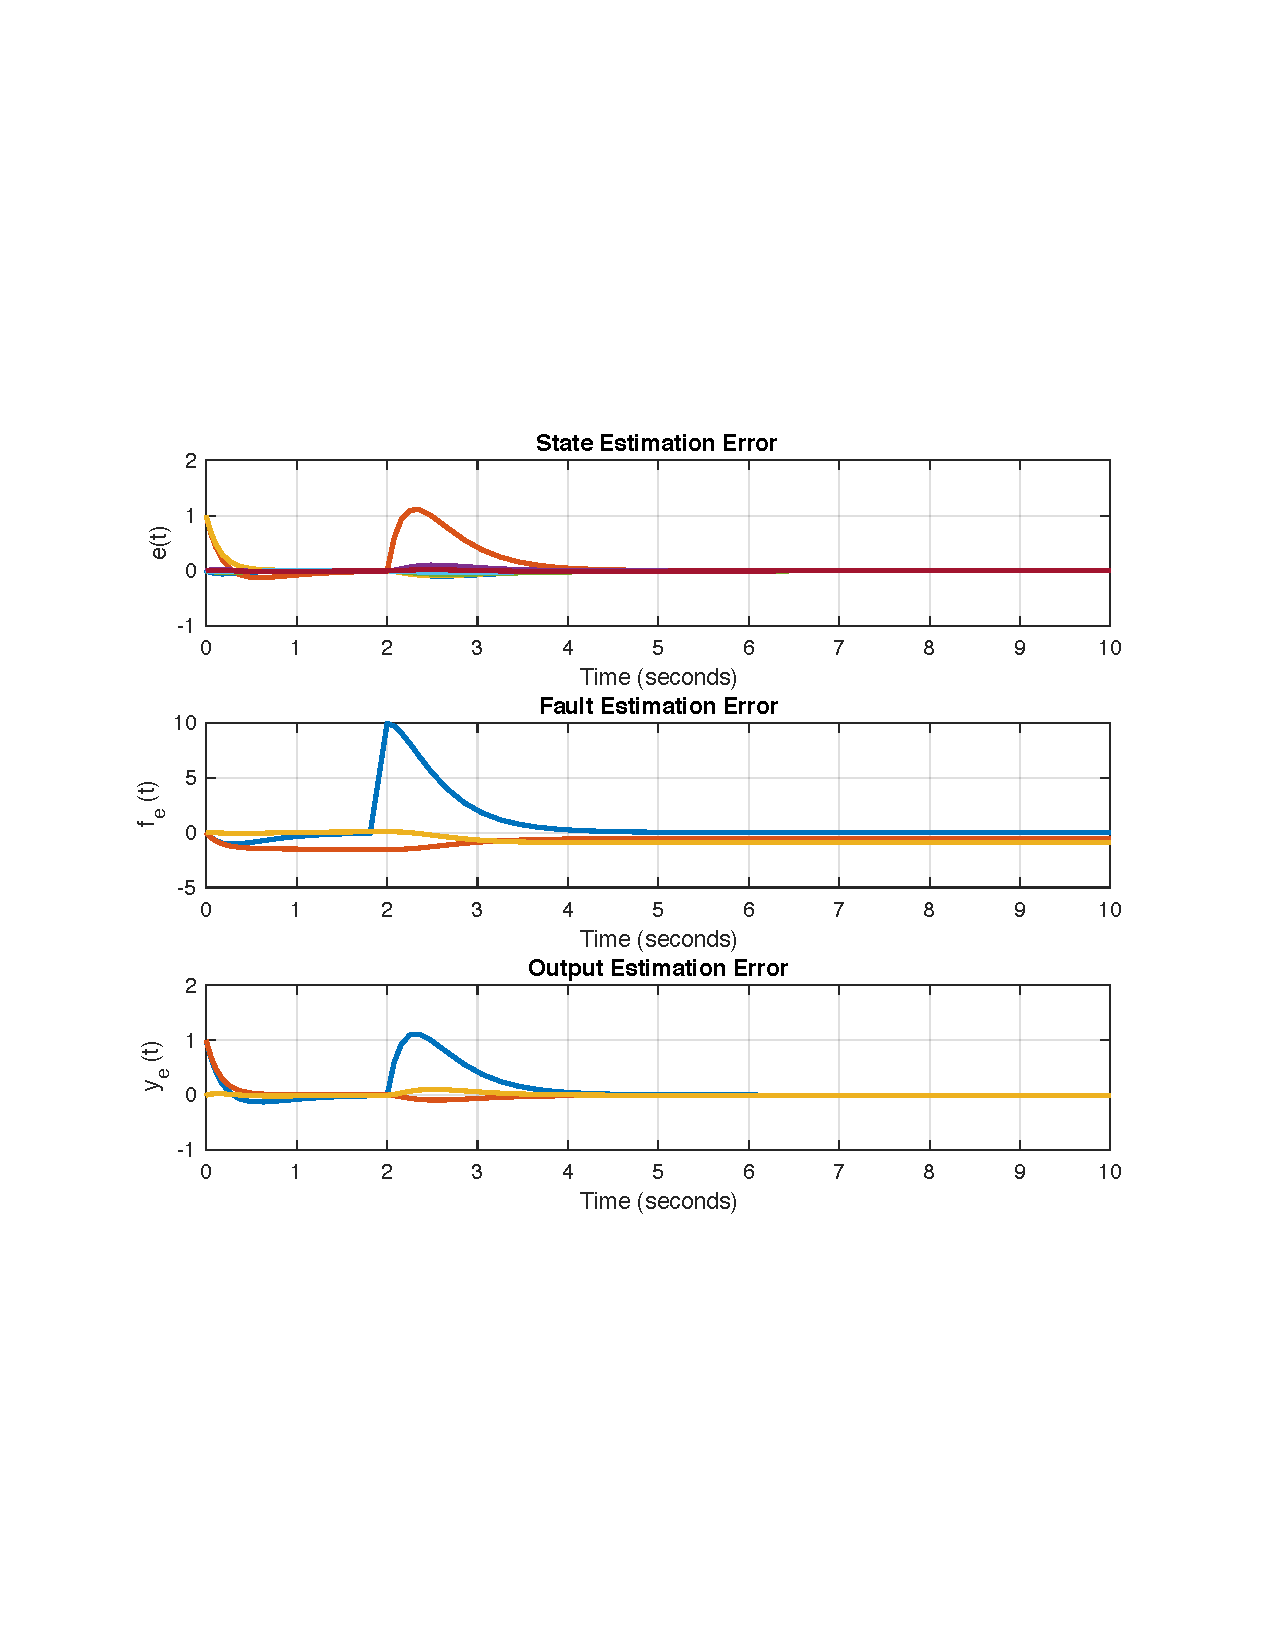
\includegraphics[scale=0.5]{images/estError.pdf}
    \caption{A plot of the state estimation error (top), fault estimation error (middle) and the output estimation error (bottom). }
    \label{fig:D_PIO_1}
\end{figure}
\begin{figure}
    \centering
    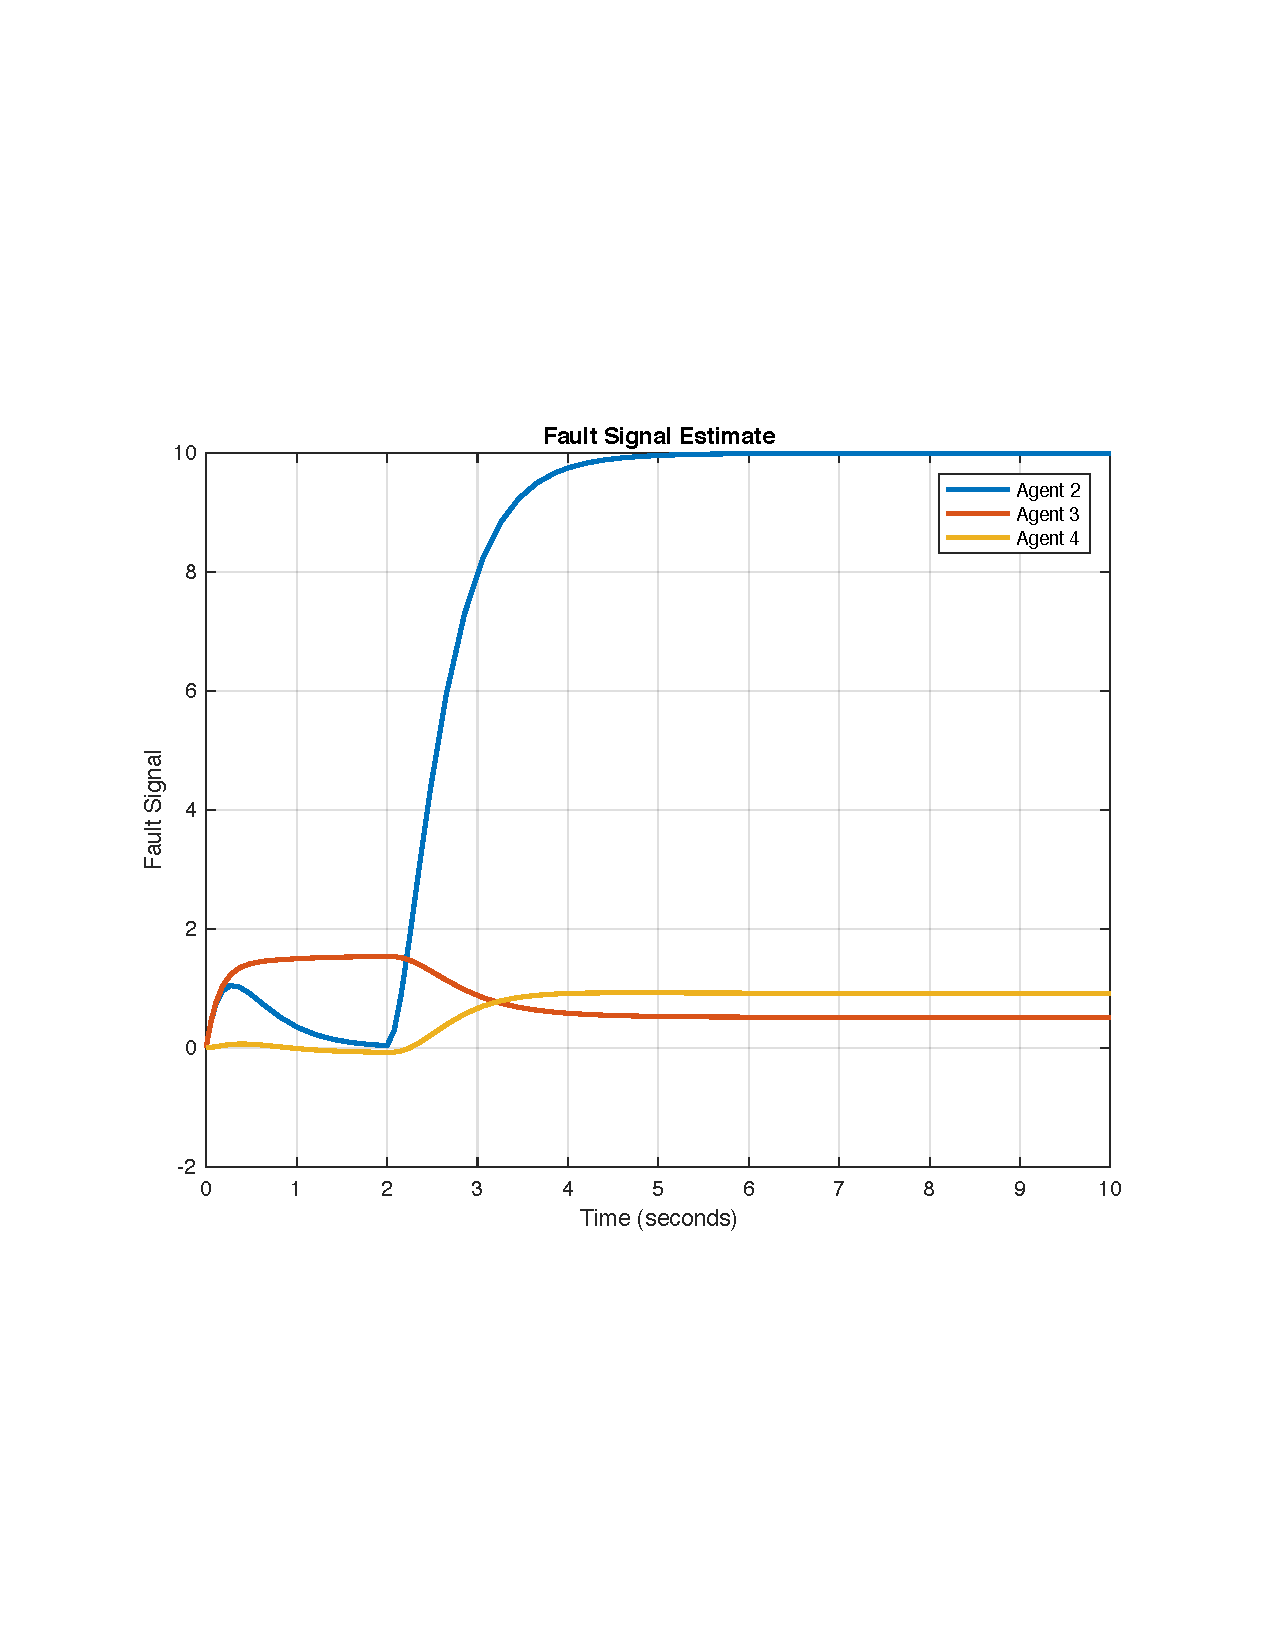
\includegraphics[scale=0.5]{images/faultEstimate.pdf}
    \caption{The residual signal which in this case is the fault estimate. As shown in blue, agent 2 experiences a fault at $t=2$. The estimated fault signal then quickly changes mean from $\mu = 0$ to $\mu = 10$.}
    \label{fig:D_PIO_2}
\end{figure}
%%%%%%%%%%%%%%%%%%%%%%%%%%%%%%%%%%%%%%%%%%%%%%%%%%%%%%%%%%%%%%%%%%%%%%%%%%%%%%%%

\section{CONCLUSION} \label{sec:con}
In this paper a distributed fault detection and isolation problem was introduced and system models for nominal and faulty conditions were derived. It was shown that the D-PIO effectively estimates the fault signal in an agent and that it can be used for residual generation and fault isolation. The conditions under which fault isolation is achievable were stated as a function of the distributed topology of the agents in the network. An LMI was obtained that can be used to compute the residual generator gains. The D-PIO design approach was illustrated with an example. 
%%%%%%%%%%%%%%%%%%%%%%%%%%%%%%%%%%%%%%%%%%%%%%%%%%%%%%%%%%%%%%%%%%%%%%%%%%%%%%%%
%\section*{APPENDIX}

%Appendixes should appear before the acknowledgment.

%\section*{ACKNOWLEDGMENT}

%%%%%%%%%%%%%%%%%%%%%%%%%%%%%%%%%%%%%%%%%%%%%%%%%%%%%%%%%%%%%%%%%%%%%%%%%%%%%%%%


% \begin{thebibliography}{99}

% \bibitem{c1} G. O. Young, ÒSynthetic structure of industrial plastics (Book style with paper title and editor),Ó 	in Plastics, 2nd ed. vol. 3, J. Peters, Ed.  New York: McGraw-Hill, 1964, pp. 15Ð64.
% \bibitem{c2} W.-K. Chen, Linear Networks and Systems (Book style).	Belmont, CA: Wadsworth, 1993, pp. 123Ð135.
% \bibitem{c3} H. Poor, An Introduction to Signal Detection and Estimation.   New York: Springer-Verlag, 1985, ch. 4.
% \bibitem{c4} B. Smith, ÒAn approach to graphs of linear forms (Unpublished work style),Ó unpublished.
% \bibitem{c5} E. H. Miller, ÒA note on reflector arrays (Periodical styleÑAccepted for publication),Ó IEEE Trans. Antennas Propagat., to be publised.
% \bibitem{c6} J. Wang, ÒFundamentals of erbium-doped fiber amplifiers arrays (Periodical styleÑSubmitted for publication),Ó IEEE J. Quantum Electron., submitted for publication.
% \bibitem{c7} C. J. Kaufman, Rocky Mountain Research Lab., Boulder, CO, private communication, May 1995.
% \bibitem{c8} Y. Yorozu, M. Hirano, K. Oka, and Y. Tagawa, ÒElectron spectroscopy studies on magneto-optical media and plastic substrate interfaces(Translation Journals style),Ó IEEE Transl. J. Magn.Jpn., vol. 2, Aug. 1987, pp. 740Ð741 [Dig. 9th Annu. Conf. Magnetics Japan, 1982, p. 301].
% \bibitem{c9} M. Young, The Techincal Writers Handbook.  Mill Valley, CA: University Science, 1989.
% \bibitem{c10} J. U. Duncombe, ÒInfrared navigationÑPart I: An assessment of feasibility (Periodical style),Ó IEEE Trans. Electron Devices, vol. ED-11, pp. 34Ð39, Jan. 1959.
% \bibitem{c11} S. Chen, B. Mulgrew, and P. M. Grant, ÒA clustering technique for digital communications channel equalization using radial basis function networks,Ó IEEE Trans. Neural Networks, vol. 4, pp. 570Ð578, July 1993.
% \bibitem{c12} R. W. Lucky, ÒAutomatic equalization for digital communication,Ó Bell Syst. Tech. J., vol. 44, no. 4, pp. 547Ð588, Apr. 1965.
% \bibitem{c13} S. P. Bingulac, ÒOn the compatibility of adaptive controllers (Published Conference Proceedings style),Ó in Proc. 4th Annu. Allerton Conf. Circuits and Systems Theory, New York, 1994, pp. 8Ð16.
% \bibitem{c14} G. R. Faulhaber, ÒDesign of service systems with priority reservation,Ó in Conf. Rec. 1995 IEEE Int. Conf. Communications, pp. 3Ð8.
% \bibitem{c15} W. D. Doyle, ÒMagnetization reversal in films with biaxial anisotropy,Ó in 1987 Proc. INTERMAG Conf., pp. 2.2-1Ð2.2-6.
% \bibitem{c16} G. W. Juette and L. E. Zeffanella, ÒRadio noise currents n short sections on bundle conductors (Presented Conference Paper style),Ó presented at the IEEE Summer power Meeting, Dallas, TX, June 22Ð27, 1990, Paper 90 SM 690-0 PWRS.
% \bibitem{c17} J. G. Kreifeldt, ÒAn analysis of surface-detected EMG as an amplitude-modulated noise,Ó presented at the 1989 Int. Conf. Medicine and Biological Engineering, Chicago, IL.
% \bibitem{c18} J. Williams, ÒNarrow-band analyzer (Thesis or Dissertation style),Ó Ph.D. dissertation, Dept. Elect. Eng., Harvard Univ., Cambridge, MA, 1993. 
% \bibitem{c19} N. Kawasaki, ÒParametric study of thermal and chemical nonequilibrium nozzle flow,Ó M.S. thesis, Dept. Electron. Eng., Osaka Univ., Osaka, Japan, 1993.
% \bibitem{c20} J. P. Wilkinson, ÒNonlinear resonant circuit devices (Patent style),Ó U.S. Patent 3 624 12, July 16, 1990. 






% \end{thebibliography}


% Our bibliography is based on http://pitt.libguides.com/citationhelp/ieee
\bibliography{Zotero.bib}
\bibliographystyle{IEEEtran}
\end{document}
